%~ Questo sorgente è stato scritto da Giovan Battista Rolandi
%~ ed è rilasciato sotto licenza GPL3

%\documentclass[handout]{beamer} %% stile di stampa su carta
\documentclass{beamer}
\usepackage[utf8]{inputenc}

\usetheme{Madrid}
%~ \usetheme{Luebeck}
%~ \usetheme{Berkeley}
%~ \usetheme{Goettingen}
%~ \usetheme{Rochester}
%~ \usetheme{Singapore}
\setbeamertemplate{caption}[numbered]
\setbeamercovered{dynamic}
\renewcommand{\figurename}{Figura}

\title{Introduzione a GPG}
\subtitle{GNU Privacy Guard: proteggere le proprie comunicazioni da sguardi indiscreti}
\author{giomba}
\date{24 Ottobre 2015}
\institute{GOLEM Empoli}

\begin{document}

\begin{frame}
  \maketitle
  \tableofcontents
\end{frame}

\begin{frame}
  \frametitle{Problema}
  Comunicare in maniera sicura e impedire la lettura dei messaggi
  alle persone non autorizzate.

  \pause
  \begin{exampleblock}{Esempi}
    \begin{itemize}
      \item Durante una guerra, impedire al nemico di leggere le comunicazioni militari
      \item Durante un acquisto online, impedire ad un ladro di intercettare il numero della nostra carta di credito
      \item ...
    \end{itemize}
  \end{exampleblock}
\end{frame}

\begin{frame}
  \frametitle{Soluzioni}

  \begin{block}{Soluzioni}
    \begin{description}
      \item[Steganografia]<1-> nascondere il messaggio
        \begin{minipage}{.9\linewidth}
          \begin{exampleblock}{Esempio}
            Riproduzione leggermente alterata di un'immagine, di un suono,
            di una fotografia, della traccia di un disco, ...
          \end{exampleblock}
        \end{minipage}
      \item[Crittografia]<2-> modificare la natura del messaggio
        \begin{minipage}{.9\linewidth}
          \begin{exampleblock}{Esempio}
            Sostituzione delle lettere con simboli o altre lettere, secondo
            criteri prestabiliti con l'interlocutore,
            come nei cifrari alfabetici (Cesare, Leon Battista Alberti, Enigma)
            e nei cifrari perfetti (Vernam)
          \end{exampleblock}
        \end{minipage}
    \end{description}
  \end{block}
\end{frame}

\begin{frame}
  \frametitle{Steganografia}

  \begin{minipage}{.45\linewidth}
    \begin{figure}
      \centering
      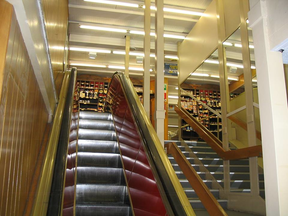
\includegraphics[width=.9\linewidth]{img/mrhyde-foto0.png}
      \caption{Originale}
      \label{fig:steg0}
    \end{figure}
  \end{minipage}
  \hfill
  \visible<2->{
    \begin{minipage}{.45\linewidth}
      \begin{figure}
        \centering
        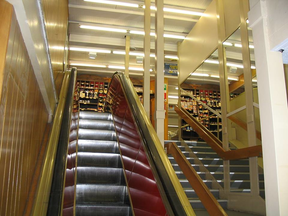
\includegraphics[width=.9\linewidth]{img/mrhyde-foto1.png}
        \caption{Steganografata}
        \label{fig:steg1}
      \end{figure}
    \end{minipage}
  }
\end{frame}

\begin{frame}
  \frametitle{Crittosistema: il Cifrario Perfetto}

  \begin{block}{Definizione}
    La probabilità di determinare quale sia il messaggio originale non
    dipende dalla conoscenza del messaggio cifrato.
  \end{block}

  \begin{minipage}{.25\linewidth}
    \begin{figure}
      \centering
      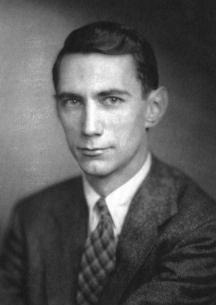
\includegraphics[width=.9\linewidth]{img/shannon.jpeg}
      \caption{Claude~Shannon}
      \label{fig:shannon}
    \end{figure}
  \end{minipage}
  \pause
  \hfill
  \begin{minipage}{.70\linewidth}
    \begin{block}{Problemi}
      \begin{itemize}
        \item La chiave di cifratura deve essere completamente casuale
        \item La chiave deve essere lunga almeno quanto il messaggio
        \item La chiave può essere utilizzata solamente una volta
        \item Non è garantita l'autenticità del messaggio ricevuto
        \item<3-> La chiave deve essere trasmessa attraverso un mezzo sicuro
      \end{itemize}
    \end{block}
  \end{minipage}

\end{frame}

\begin{frame}
  \frametitle{Crittosistema: Crittografia Asimmetrica}
  \framesubtitle{Una cifratura accettabile}

  \begin{block}{Svantaggi}
    Non è perfetto
  \end{block}

  \begin{exampleblock}{Cosa significa?}
  Avendo a disposizione una notevole capacità di calcolo e un lunghissimo tempo,
  si può recuperare il messaggio.
  \end{exampleblock}

  \pause
  \begin{block}{Vantaggi}
    \begin{itemize}
      \item non può essere decifrato in tempi ragionevolmente utili;
      \item è necessario scambiarsi la chiave una volta sola,
      \item e non è necessario un mezzo di comunicazione sicuro;
      \item la chiave può essere essere utilizzata infinite volte;
      \item è possibile autenticare il mittente.
    \end{itemize}
  \end{block}

\end{frame}

\begin{frame}
  \frametitle{Crittografia asimmetrica: GPG GNU Privacy Guard}
  \framesubtitle{Un'implementazione libera di un algoritmo di crittografia asimmetrica}

  \begin{block}{Come funziona in pratica?}
    \centering
    
\includegraphics[width=.9\linewidth]{img/ab0.pdf}
  \end{block}
\end{frame}

\begin{frame}
  \frametitle{Crittografia asimmetrica: GPG GNU Privacy Guard}
  \framesubtitle{Un'implementazione libera di un algoritmo di crittografia asimmetrica}

  \begin{block}{Come funziona in pratica?}
    \centering
    
\includegraphics[width=.9\linewidth]{img/ab1.pdf}
  \end{block}
\end{frame}

\begin{frame}
  \frametitle{Crittografia asimmetrica: GPG GNU Privacy Guard}
  \framesubtitle{Un'implementazione libera di un algoritmo di crittografia asimmetrica}

  \begin{block}{Come funziona in pratica?}
    \centering
    
\includegraphics[width=.9\linewidth]{img/ab2.pdf}
  \end{block}
\end{frame}

\begin{frame}
  \frametitle{Crittografia asimmetrica: GPG GNU Privacy Guard}
  \framesubtitle{Un'implementazione libera di un algoritmo di crittografia asimmetrica}

  \begin{block}{Come funziona in pratica?}
    \centering
    
\includegraphics[width=.9\linewidth]{img/ab3.pdf}
  \end{block}
\end{frame}

\begin{frame}
  \frametitle{Crittografia asimmetrica: GPG GNU Privacy Guard}
  \framesubtitle{Un'implementazione libera di un algoritmo di crittografia asimmetrica}

  \begin{block}{Come funziona in pratica?}
    \centering
    
\includegraphics[width=.9\linewidth]{img/ab4.pdf}
  \end{block}
\end{frame}

\begin{frame}
  \frametitle{Crittografia asimmetrica: GPG GNU Privacy Guard}
  \framesubtitle{Un'implementazione libera di un algoritmo di crittografia asimmetrica}

  \begin{block}{Come funziona in pratica?}
    \centering
    
\includegraphics[width=.9\linewidth]{img/ab5.pdf}
  \end{block}
\end{frame}

\begin{frame}
  \frametitle{Utilità}
  \framesubtitle{Ma ho davvero bisogno di tutto questo?}

  \begin{block}{Abbiamo tutti qualcosa da nascondere}
    \begin{itemize}
      \item Origine razziale ed etnica
      \item Convinzioni religiose e filosofiche
      \item Orientamento politico
      \item Orientamento sessuale
      \item Stato di salute
    \end{itemize}
  \end{block}

  \pause
  \begin{alertblock}{Meglio prevenire che curare}
    Anche se oggi, probabilmente, non ce n'è bisogno, non fa sicuramente
    male prendere confidenza con questi utili strumenti.
  \end{alertblock}
\end{frame}

\begin{frame}[fragile]
  \frametitle{GPG mini How-to}

  \begin{block}{GnuPG}
    \begin{itemize}[<+->]
      \item \tt gpg --gen-key
      \item \tt gpg --list-keys --fingerprint
      \item \tt gpg -o file.txt.gpg -e -r user@example.org file.txt
      \item \tt gpg -o file.txt -d file.txt.gpg
      \item \tt gpg --keyserver pgp.mit.edu --send-key <ID>
      \item \tt gpg --keyserver pgp.mit.edu --recv-key <ID>
      \item \tt gpg --edit-key
      \begin{itemize}
        \item \tt > fpr
        \item \tt > sign
        \item \tt > save
      \end{itemize}
    \end{itemize}
  \end{block}
\end{frame}

\begin{frame}
  \frametitle{GPG: Interfacce grafiche}
  \framesubtitle{Thunderbird + Enigmail}

  \begin{figure}
    \centering
    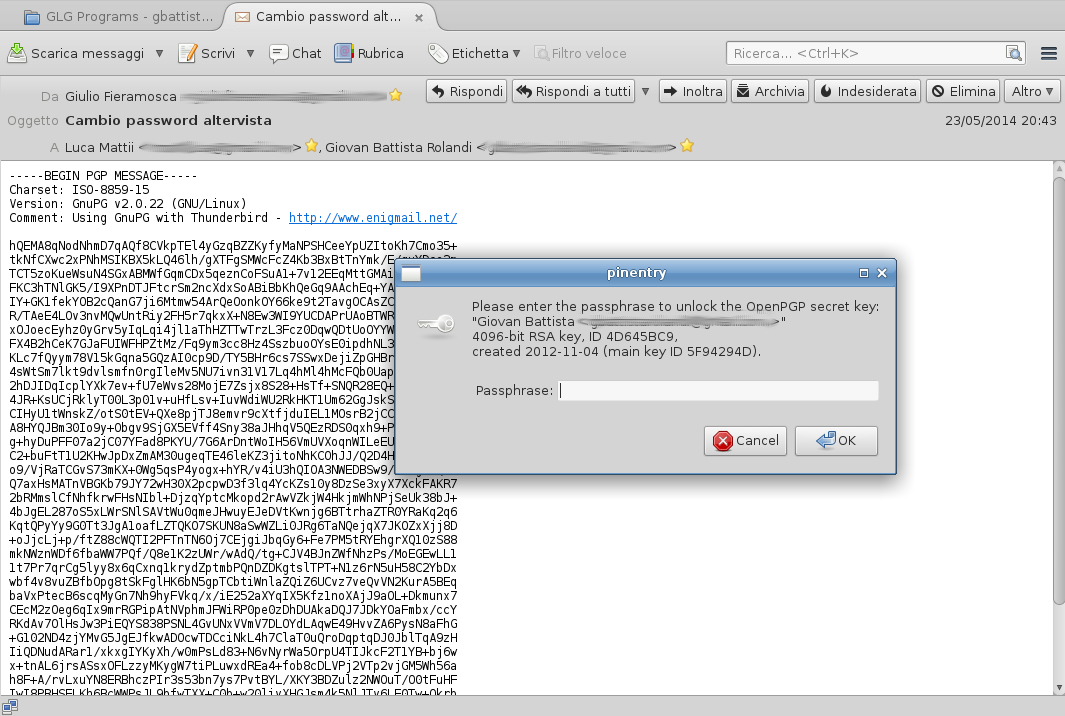
\includegraphics[width=.7\linewidth]{img/enigmail.png}
    \caption{Enigmail}
    \label{fig:enigmail0}
  \end{figure}
\end{frame}

\begin{frame}
  \frametitle{GPG: Interfacce grafiche}
  \framesubtitle{GNOME Seahorse}

  \begin{figure}
    \centering
    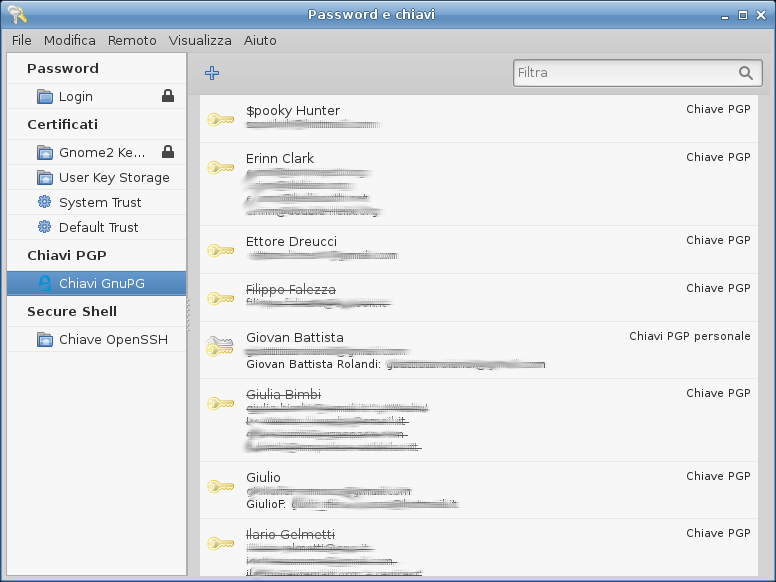
\includegraphics[width=.6\linewidth]{img/seahorse.png}
    \caption{Seahorse}
    \label{fig:seahorse0}
  \end{figure}
\end{frame}

\begin{frame}
  \frametitle{L'anello debole della catena}
  \framesubtitle{Il problema è tra la tastiera e la sedia}

  \begin{figure}
    \centering
    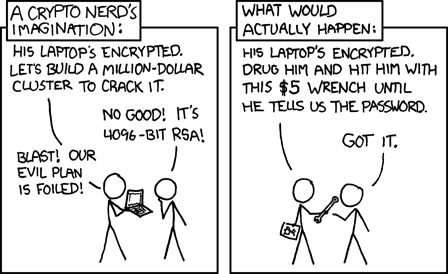
\includegraphics[width=.6\linewidth]{img/538.png}
    \caption{Security: http://xkcd.com/538}
    \label{fig:xkcd}
  \end{figure}

\end{frame}

\begin{frame}
  \frametitle{GPG Party}
  \framesubtitle{Scambio e firma di chiavi per la creazione di una rete di fiducia}

  \begin{block}{Che fare?}
    Andate, generate, e scambiatevi l'impronta di chiave.
  \end{block}

  \pause

  \begin{exampleblock}{GPG Keysignign Party: prima}
    \begin{itemize}
      \item Generare coppia di chiavi\\
            \tiny \texttt{gpg --gen-key} \normalsize
      \item Annotarsi l'impronta (\emph{fingerprint}) della propria chiave\\
            \tiny \texttt{gpg --fingerprint <ID>} \normalsize
      \item Preparare bigliettini col proprio nome, indirizzo email
            ID e impronta della propria chiave
      \item Inviare chiave pubblica ad un server\\
            \tiny \texttt{gpg --keyserver pgp.mit.edu --send-key <ID>} \normalsize
    \end{itemize}
  \end{exampleblock}

\end{frame}

\begin{frame}
  \frametitle{GPG Party}
  \framesubtitle{Scambio e firma di chiavi per la creazione di una rete di fiducia}

  \begin{exampleblock}{GPG Keysigning Party: durante}
    \begin{itemize}
      \item Recarsi ad un \emph{GPG Keysigning Party} con i bigliettini
            e muniti di documento di identità
      \item Scambiarsi la chiave con i presenti, controllando la loro identità
    \end{itemize}
  \end{exampleblock}

  \pause

  \begin{exampleblock}{GPG Keysigning Party: dopo}
    \begin{itemize}
      \item Tornare a casa \tiny \texttt{cd \~} \normalsize
      \item Scaricare le chiavi
            \tiny \texttt{gpg --keyserver pgp.mit.edu --recv-key <ID>} \normalsize
      \item Controllare la \emph{fingerprint}
            \tiny \texttt{gpg --fingerprint <ID>} \normalsize
      \item Firmare\\
            \tiny \texttt{gpg --edit-key <ID>\\ > sign} \normalsize
      \item Rispedire al server
            \tiny \texttt{gpg --keyserver pgp.mit.edu --send-key <ID>} \normalsize
    \end{itemize}
  \end{exampleblock}

\end{frame}

\begin{frame}
  \frametitle{GPG GNU Privacy Guard}

  \begin{block}{Licenza}
    \centering
    \begin{minipage}{.18\linewidth}
      \begin{figure}
        \centering
        
\includegraphics[width=.9\linewidth]{img/gnu.pdf}
      \end{figure}
    \end{minipage}
    \hfill
    \begin{minipage}{.6\linewidth}
      \centering
      Il sorgente di questa presentazione\\
      è software libero,\\
      viene rilasciato sotto licenza GPLv3,\\
      ed è consultabile presso golem.linux.it
    \end{minipage}
    \hfill
    \begin{minipage}{.18\linewidth}
      \begin{figure}
        \centering
        
\includegraphics[width=.9\linewidth]{img/gpl3.pdf}
      \end{figure}
    \end{minipage}

  \end{block}

  \begin{block}{Linux Day @ Empoli 2015}
    \centering
    \begin{minipage}{.1\linewidth}
      
\includegraphics[width=.9\linewidth]{img/GOLEM-logo.pdf}
    \end{minipage}
    \begin{minipage}{.7\linewidth}
    \centering
    Questa presentazione è stata preparata per\\
    GOLEM - golem.linux.it\\
    in occasione del Linux Day 2015\\
    da Giovan Battista Rolandi (giomba)\\
    gbattistarolandi@gmail.com\\
    GPG Public ID: 5F94294D
    \end{minipage}
    \begin{minipage}{.1\linewidth}
      
\includegraphics[width=.9\linewidth]{img/linuxday-logo.png}
    \end{minipage}
  \end{block}

\end{frame}

\end{document}
